\documentclass{article}
% All latex files should begin with a "documentclass" declaration.

% By the way, the "comment character" in latex is the percent sign.  So, anything after a % on a line will be ignored when compiling the source document.  We'll use that a lot, and you may want to use it to leave yourself notes as you're learning.  A good text editor will display comments in a different color or font, so that it's obvious what is latex and what is notes.

% All latex commands begin with a backslash, \.  Curly braces { } contain mandatory arguments to a command.  Square brackets [ ] contain optional arguments.

% For example, try editing the first line to read instead:\documentclass[12pt]{article}
% Providing that optional argument to the documentclass command changes the font size from the default (10 point) to 12 point.

% Here is much more (totally optional) information about documentclass: http://texblog.org/2013/02/13/latex-documentclass-options-illustrated/

%%%%%%%%%%%%%%%%
%%% PREAMBLE %%%
%%%%%%%%%%%%%%%%

% The preamble is a set of formatting instructions, which you provide to latex before your actual content.  It begins with the \documentclass command, above.  Then typically a lot of packages are loaded, and maybe some other declarations.  All of that can be typed right here.

% Alternatively, it can be helpful to confine much of the preamble to a separate file.  This keeps it out of your way and makes it easy to reuse for other documents.  Here, I've put most of the preamble into a separate file, which we'll load now:
\usepackage{tutorial}  % loads the tutorial.sty file
% You can take a look in tutorial.sty now, and we'll refer to it later on.

% But just to illustrate that formatting commands can be given here in the main document, try uncommenting one of these next lines (that is, remove the comment % from the beginning of the line).  This will change the font throughout the document, from LaTeX's classic Computer Modern to something else.
%
%\usepackage{mathptmx}     % Times font, for text and math
%\usepackage[sc]{mathpazo} % snazzy font suggested by American Naturalist

\title{Yet Another \LaTeX\ Tutorial}
\author{For Foundations Class}
\date{2 December 2015}

\begin{document} %  Essential!  And don't forget the matching \end{document} at the end of your content.

\maketitle
% This goes with the \title{} above.  There is lots more about titlepages here: https://en.wikibooks.org/wiki/LaTeX/Title_Creation

%%%%%%%%%%%%%%%%%
%%% MAIN TEXT %%%
%%%%%%%%%%%%%%%%%

Each section below highlights features or commands in \LaTeX.
Each ends with a suggestion for experimenting with what you've just learned.
Definitely feel free to experiment more!

%--------------------------------------------------
\section{If Using Overleaf} % This is the name of this section, obviously.
\label{sec:overleaf}        % This \label command is optional.  See the Cross-Reference section below for an explanation.
%--------------------------------------------------

Before we start, here are a few preliminaries that will make things easier if you're using this tutorial through the Overleaf web service.

\begin{enumerate}
    \item Copy the URL to somewhere.  This will allow you to retain any changes you make.
    \item Switch the Preview button from Auto to Manual.  This will prevent unnecessary compilation when you're not ready for it.  To compile the document after you've made changes, click ``refresh preview.''
    \item Click Versions and create a label for this original state of the document.  This will make it easy to see what you've changed.
\end{enumerate}

(By the way, each Overleaf project is secretly a git repository!
So you can push and pull your changes instead of editing in a web browser.
We won't get into that here, though.)
% https://www.overleaf.com/blog/195-new-collaborate-online-and-offline-with-overleaf-and-git-beta

%--------------------------------------------------
\section{Lists}
\label{sec:lists}
%--------------------------------------------------

We've already used a list above.
In general, a \latexcode{\\begin} command must always have a matching \latexcode{\\end} command.
Above, we began and ended an \latexcode{enumerate} environment to get a numbered list.
Each item in the list begins with \latexcode{\\item}.

Here is a nested list:
\begin{enumerate}
    \item Plant
    \begin{enumerate}
        \item Tomato
        \item Hosta
    \end{enumerate}
    \item Animal
    \begin{enumerate}
        \item Cat
        \item Stegosaurus
    \end{enumerate}
\end{enumerate}

\subsection{\task}

Copy or type a numbered list here, with a third layer of nesting.

Change the list to use bullet points instead of numbers, by changing \latexcode{enumerate} to \latexcode{itemize}.

%--------------------------------------------------
\section{Paragraphs}
\label{sec:paragraphs}
%--------------------------------------------------

Paragraphs are separated by blank lines in the source file, as you have probably realized by now.
If there is no blank line, the text is all formatted as the same paragraph.
Thus, \LaTeX\ ignores the linebreak that comes at the end of each sentence here.
One sentence per line is good practice, though, especially when using version control (like git).

Here is the start of a new paragraph.  \\
The double-backslash causes this sentence to start on a new line, but without a paragraph break.

\vspace{20pt}
Adding more blank lines doesn't increase the amount of space between paragraphs.
To do that, we use the \latexcode{\\vspace} command to add a specified amount of vertical space.

Here are some miscellaneous examples of text formatting.
\textbf{Bold.}
\emph{Emphasized.  Usually italic.  But can be un-italicized if \emph{emphasized} within italics.}
\texttt{Typewriter-style text.}
\large{Larger than usual.}
\small{Smaller than usual.}
`Inside single smart quotes.'
``Inside double smart quotes---it's an em-dash!''

\subsection{\task}

Write two paragraphs of text.
Try to stick with one line per sentence.
Use unnecessary text formatting (bold, etc.)

Adjust the paragraph indentation and spacing between paragraphs by changing the values of \latexcode{\\parindent} and \latexcode{\\parskip} in \latexcode{tutorial.sty}.

Notice how nice the justified text looks.
But to remove the right justification, find the \latexcode{\\raggedright} command in \latexcode{tutorial.sty}.

%--------------------------------------------------
\section{Custom Commands}
\label{sec:custom}
%--------------------------------------------------

Now let's jump straight to an advanced \LaTeX\ feature: defining your own commands.
We've already used two of them, which I put into \latexcode{tutorial.sty}.
One is \latexcode{\\latexcode}, for printing \LaTeX\ commands without executing them---it's a bit complicated, so don't mess with that line.

\subsection{\task}

The other custom command is simpler, and you can easily change it.
I wanted each subsection of exercises to have the same name, but I kept changing my mind about what that name should be.
It is currently \task.
Go into \latexcode{tutorial.sty}, find the line where \latexcode{\\task} is defined, and change the definition to something else, maybe ``Exercises'' or ``Tasks''.
Now notice the new name of this subsection, and of all the other ones with tasks.
This is a handy trick to maintain consistency without repeated bouts of search-and-replace.

%--------------------------------------------------
\section{Sections}
\label{sec:sections}
%--------------------------------------------------

We have also defined in \latexcode{tutorial.sty} how the section headings should look, using the \latexcode{titlesec} package.

\subsection{This is a Subsection}

\subsubsection{This is a Subsubsection}

\subsubsection*{This is a Subsubsection Without a Number}

We can refer to sections by number, even if we don't know what the number is.
For example, we discussed custom commands in \cref{sec:custom}, and we are now discussing sections in \cref{sec:sections}.
We'll talk about cross-referencing more below (\cref{sec:refs}), but for now, just know that the key was the \latexcode{\\label} command we issued right after the name of each section.

\subsection{\task}

In \latexcode{tutorial.sty}, change the subsubsection format to small caps.
Look at the lines above to check that it worked.

Refer by number to the section where we discussed paragraph formatting.

%--------------------------------------------------
\section{Math}
\label{sec:math}
%--------------------------------------------------

Math typesetting is where \TeX\ shines.
Inline math is denoted with \latexcode{\$}.
For example, $\alpha_z = 1$ but $\Gamma^2 = \sqrt{7 y}$.

Display math works like this:
\begin{equation}
    \frac{d}{dx} \left( \int_{0}^{x} f(u)\, du \right) = f(x)
\label{eq:deriv}
\end{equation}

% Here is a ton more info on math typesetting:
%     https://en.wikibooks.org/wiki/LaTeX/Mathematics
%     http://mirrors.ctan.org/macros/latex/required/amslatex/math/amsldoc.pdf

\subsection{\task}

The quadratic equation is
\begin{equation}
    a x^2 + b x + c = 0.
\label{eq:quadratic}
\end{equation}
Write out its solution for x.
% Hint: https://en.wikipedia.org/wiki/Quadratic_formula

%--------------------------------------------------
\section{Literature Citations}
\label{sec:literature}
%--------------------------------------------------

For in-text citations and printing the list of literature cited, \LaTeX\ uses BibTeX.
(Or BibLaTeX is the new implementation, but I have not figured out how to use that with our journals.)
See the \latexcode{refs.bib} file for the papers that are cited in the following paragraph.

\citet{Janzen1967} started his paper with a reference to \citet{Simpson1964}, who noted that restricted dispersal should lead to increased population isolation and hence an increased number of species.
The difficulty of crossing mountain barriers in less seasonal environments, Janzen argued, may therefore contribute to the higher species diversity in tropical regions than temperate ones \citep{Ghalambor2006}.
This falls into one general class of explanations for why there are more species at lower latitudes: that there is a higher rate of lineage diversification (speciation minus extinction) in tropical regions               \citep{Ricklefs2006, Weir2007, Mittelbach2007}.

Along with BibTeX, we're using the package \latexcode{natbib} to format the citations, and the bibliography style file \latexcode{amnatnat.bst} (provided by \emph{American Naturalist}) to format the references section.
% https://en.wikibooks.org/wiki/LaTeX/Bibliography_Management#BibTeX
% https://en.wikibooks.org/wiki/LaTeX/Bibliography_Management#Natbib
The References would normally be printed at the end of the document, but let's put them here for convenience.

\bibliography{refs}          % see refs.bib
\bibliographystyle{amnatnat} % see amnatnat.bst

\subsection{\task}

Add one paper to \latexcode{refs.bib}.
You can type in all the info, or look for an ``Export to BibTeX'' link on a journal webpage or Google Scholar.
When you recompile this document, do you see your new paper in the References section above?

Now write a sentence that cites your new paper, and then recompile this document.
Now do you see your new reference in the References above?

%--------------------------------------------------
\section{Figures}
\label{sec:figures}
%--------------------------------------------------

The \latexcode{\\includegraphics} command can be used to place an image in your document.
Usually, however, we want to package a caption along with the figure.
When \LaTeX\ does this, it places the figure+caption into a ``floating'' container, so that they occur together and are placed somewhere that is nearby and suits the page layout.
% https://en.wikibooks.org/wiki/LaTeX/Floats,_Figures_and_Captions

For example, I am writing the info for \cref{fig:landscape} here, but it may be placed elsewhere on this or the the following page if it fits better there.
\begin{figure}
\centering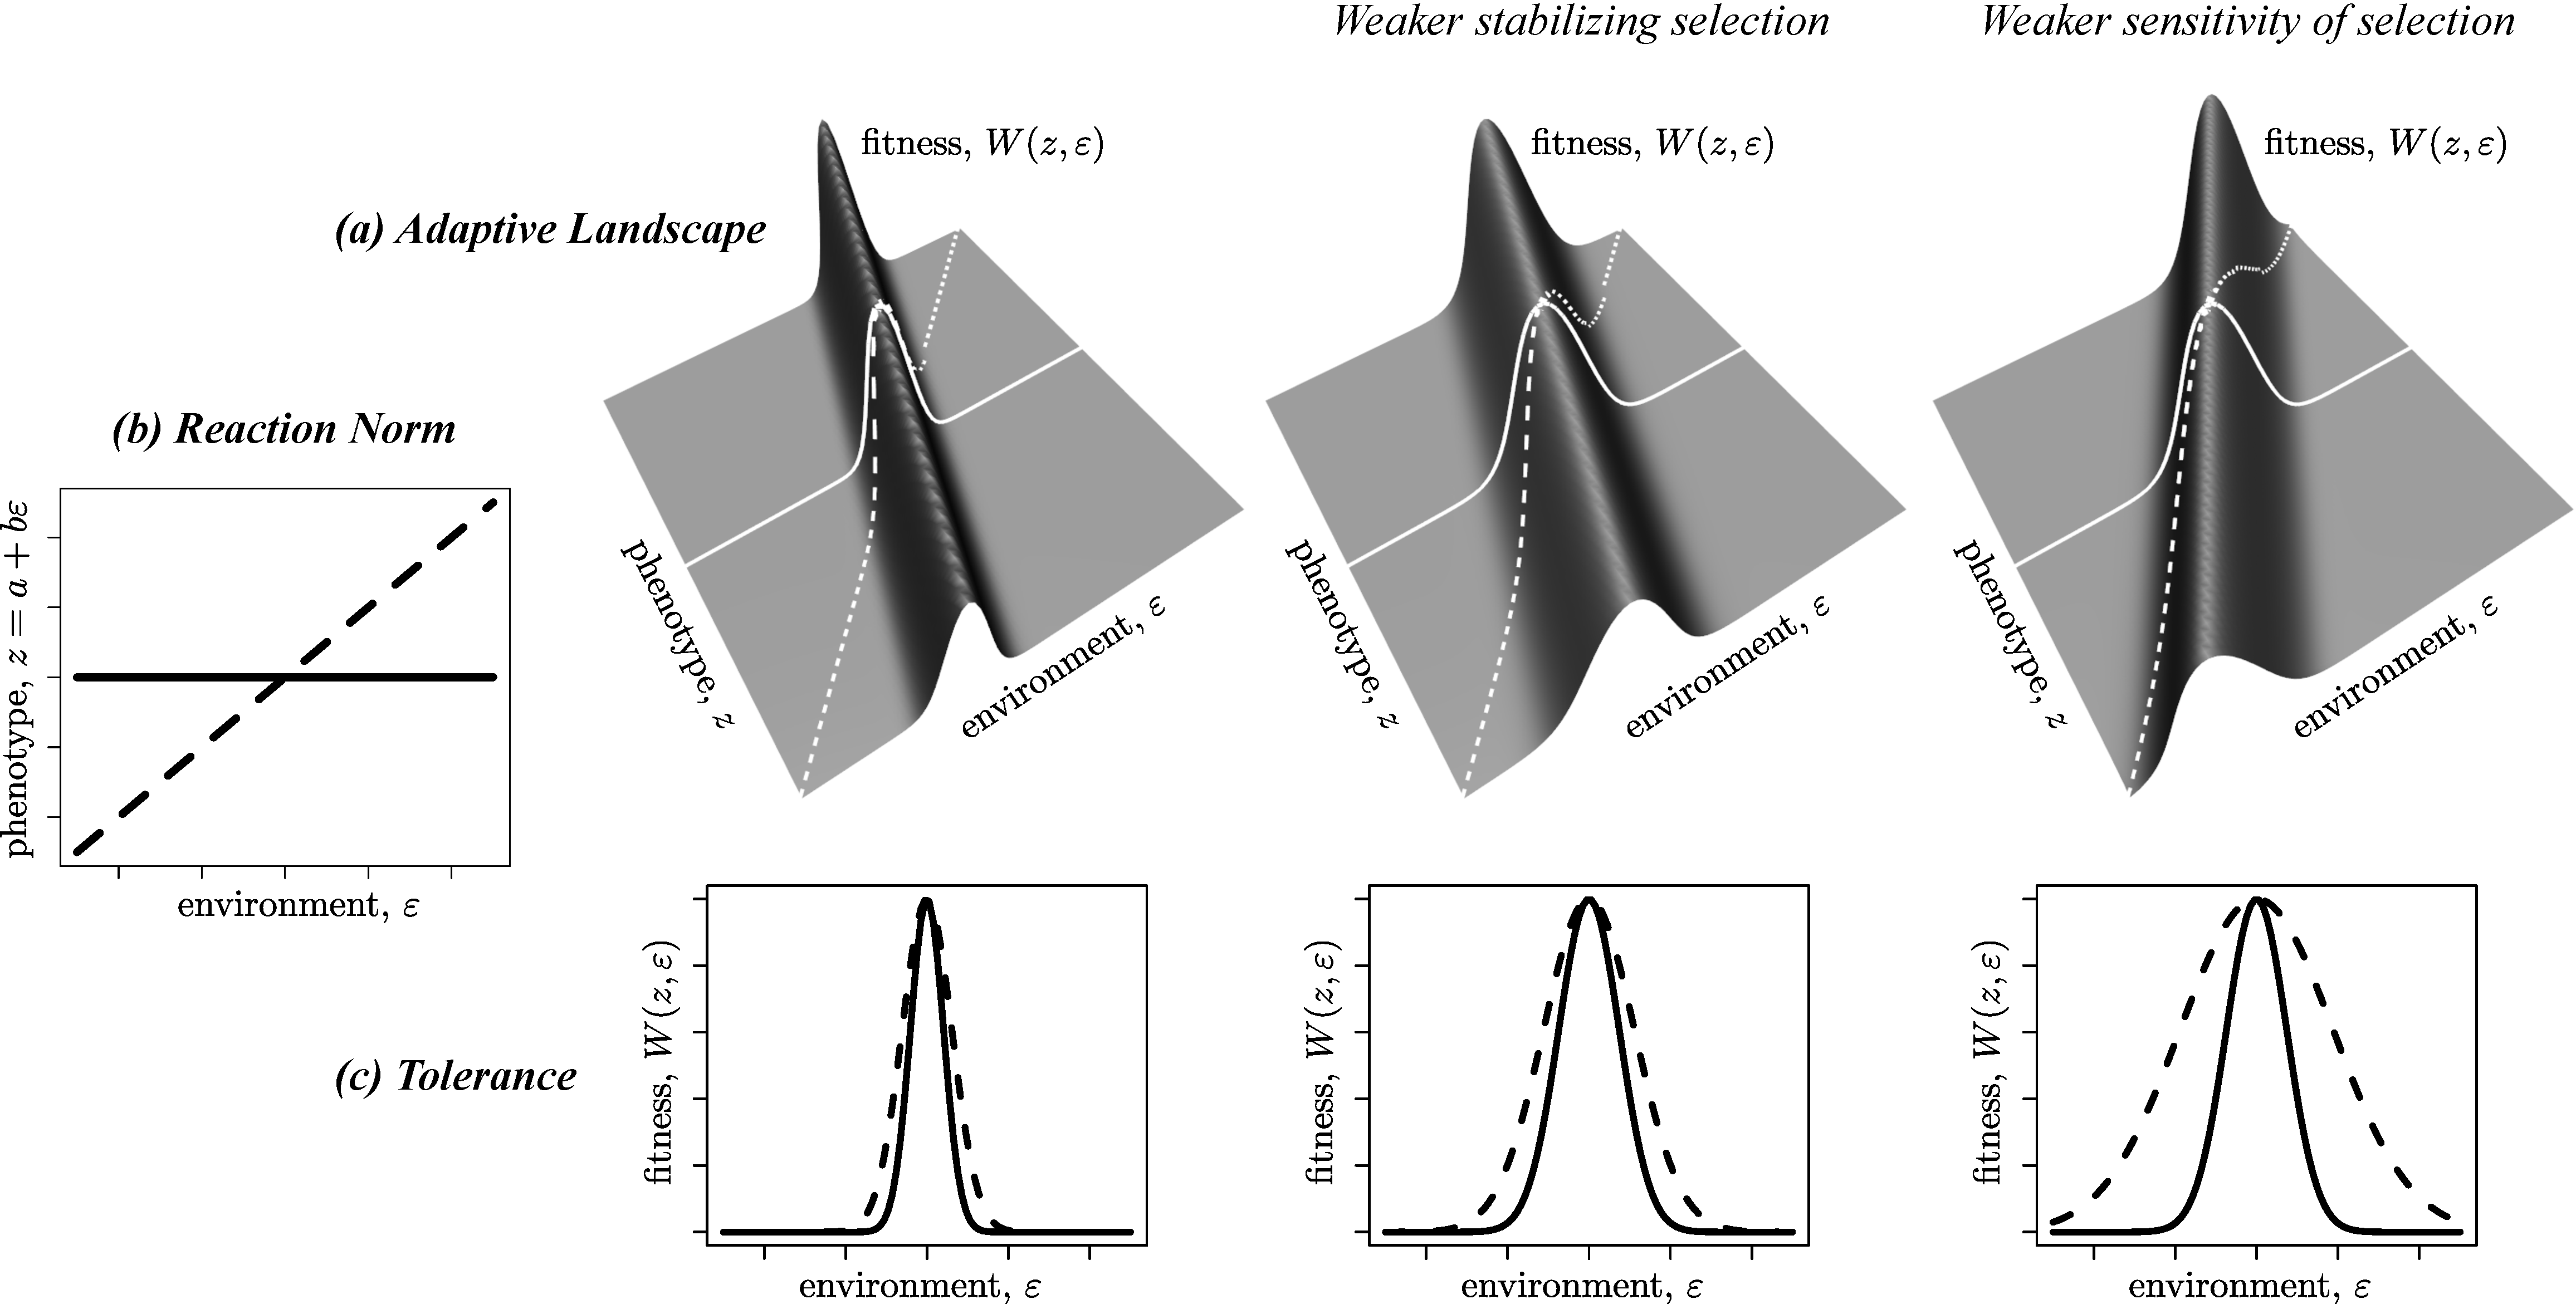
\includegraphics[width=0.8\textwidth]{landscape.pdf}
\caption{A generalized adaptive landscape.
    This is here because it was the first PDF figure I found.
    \LaTeX\ can handle lots of graphics formats, but PDF is especially nice because it is a vector format and so scales well.
    By the way, Inkscape is fantastic (and free) software for making vectorized figures and diagrams.
}
\label{fig:landscape}
\end{figure}

This subsequent figure, \cref{fig:lion}, will definitely be placed after the earlier figure.
\begin{SCfigure}[50]
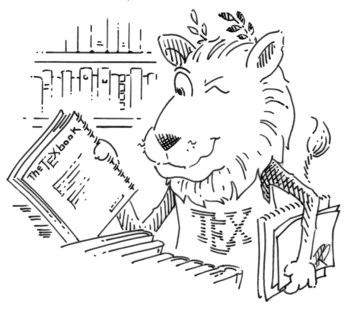
\includegraphics[width=0.25\textwidth]{lion.png}
% https://www.ctan.org/lion/
\caption{CTAN lion drawing by Duane Bibby.
    Also, this caption is to the side of the image.
    Non-standard, but sometimes useful.
}
\label{fig:lion}
\end{SCfigure}

\subsection{\task}

Add a figure and its caption.

When you have large figures and captions, and especially when a journal demands it, it's nice to have an easy way to place all the figures at the end of the document.
To accomplish this, go into \latexcode{tutorial.sty} and uncomment the code for the \latexcode{endfloat} package.
See what happens with the figure placement, and note the snazzy list of figures.

%--------------------------------------------------
\section{Cross-Referencing}
\label{sec:refs}
%--------------------------------------------------
% TODO

cref \\
section by name (number was done above) \\
equation, figure, table \\
change Figure to Fig.

\TeX\ has a classy mascot, as we see in \cref{fig:lion}.
There is also some biology in \cref{fig:landscape}.

\end{document} % Essential!  The end of your content.

(use booktabs)
tabular
table (floating env)
copy, add row, add column, align column
(R's xtable)

\include table or some text

line numbers

table of contents
